\documentclass{beamer}
\DeclareFontShape{OT1}{cmss}{b}{n}{<->ssub * cmss/bx/n}{} 
\usetheme{Szeged}
\usecolortheme{beaver}
\usepackage{amsmath}
\usepackage{amsfonts}
\usepackage{mathbbol}
\usepackage{xcolor} % before tikz or tkz-euclide if necessary
\usepackage{tkz-euclide} % no need to load TikZ
\usepackage{multirow}
\usepackage{lmodern}
\usepackage{bm}
\usepackage{subcaption}
%\usepackage{subfigure}

\usepackage[
backend=biber,
style=authoryear-icomp,
sortlocale=de_DE,
natbib=true,
url=false, 
doi=true,
eprint=false
]{biblatex}
\addbibresource{../Bibliography/main_ML.bib}



\titlegraphic{
\includegraphics[width=2cm]{../Figures/UAMS_RGB.png}
}


\title{Neuroinformatics Journal Club\\ Dynamic Mode Decomposition }
\author{Horacio G\'omez-Acevedo\\ Department of Biomedical Informatics\\
	University of Arkansas for Medical Sciences}

\begin{document}
	\begin{frame}[plain]
		\maketitle
	\end{frame}
	
	\begin{frame}{Today's paper}
		\begin{figure}[h]
			\centering
			%	\begin{subfigure}{0.4\textwidth}
				%		\centering
				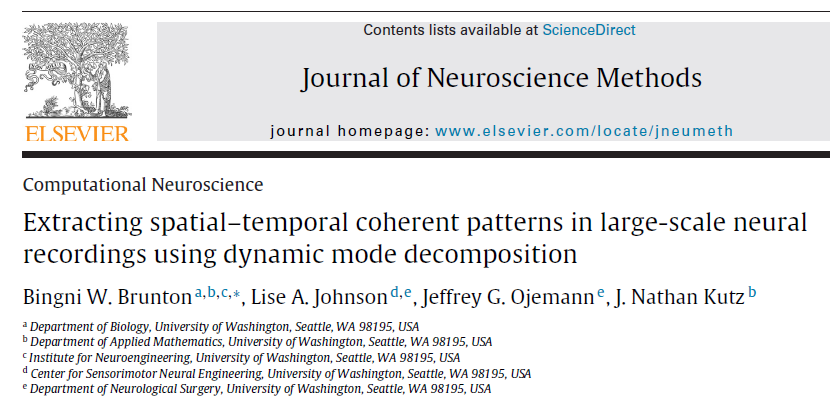
\includegraphics[scale=0.45]{../Figures/fig_brunton_paper.png}
				%	\end{subfigure}
		\end{figure}
	\end{frame}
	
	
\begin{frame}{Background}
What are eigenvalues and eigenvectors?

Let $A$ be a $n\times n$ matrix  (real), a number $\lambda \in \mathbb{C}$ is an \textbf{eigenvalue} if there is a nonzero vector $x \in \mathbb{C}^n$ for which $Ax= \lambda x$. We call such a vector an \textbf{eigenvector} of $A$ associated with $\lambda$. 

The collection of all eigenvalues of $A$ is called the \textbf{spectrum} of $A$.

The fundamental theorem for linear systems: If $A$ is a $n\times n$ matrix. For any $x_0 \in \mathbb{R}^n$, the initial value problem 
\begin{equation*}
	\dot{x}=A x \qquad x(0)=x_0
\end{equation*}
has a unique solution
\begin{equation*}
	x(t)= \exp(A^t)x_0
\end{equation*}

\end{frame}


	\begin{frame}{Eigenvalues in Dynamical Systems}
		\begin{figure}[h]
	\centering
	%	\begin{subfigure}{0.4\textwidth}
		%		\centering
		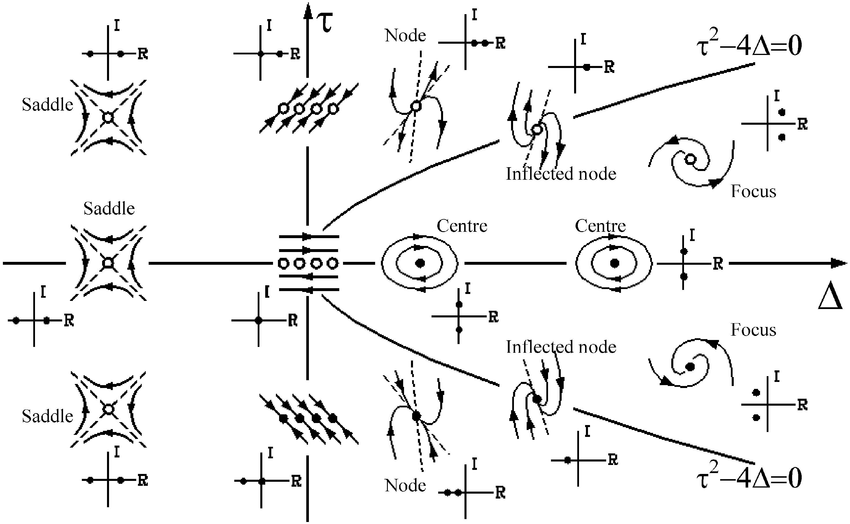
\includegraphics[scale=0.3]{../Figures/fig_phase_portrait.png}
		%	\end{subfigure}
\end{figure}
\url{https://www.researchgate.net/profile/Marco-Altosole/publication/245387409/figure/fig1/AS:392836487892996@1470670925920/Types-of-phase-portrait.png}		
	\end{frame}

\begin{frame}{Singular Value Decomposition}
	If $A \in M_{m,n}$ has rank $k$, then it may be written in the form 
	\begin{equation*}
	A=V \Sigma W^*
	\end{equation*}
where $V\in M_m$ and $W\in M_n$ are unitary ($W^* W=I_n$). The matrix $\Sigma=diag\{\sigma_1,\ldots, \sigma_q\}$ are the non-negative square roots of the eigenvalues of $AA^*$. The columns of $V$ are eigenvectors of $AA^*$, and the columns of $W$ are eigenvectors of $A^* A$. If $m\le n$ and if $AA^*$ has distinct eigenvalues, then $V$ is determined up to a right diagonal factor $D=diag( \exp(i\theta_1), \ldots, \exp(i \theta_n)$ where $\theta_j \in \mathbb{R}$. 
\end{frame}

\begin{frame}{Main Premise}
	The DMD algorithm seeks a best-fit linear matrix $A$ that approximately advances the state of a system $x\in \mathbb{R}^n$ forward in time according to the linear system
	\begin{equation*}
		x_{k+1}= A x_k
	\end{equation*}
where $x_k= x(k\Delta t)$ and $\Delta t$ denotes a fixed time step that is small enough to resolve the highest frequencies in the dynamics.
\end{frame}

\begin{frame}{DMD setup }
	\begin{figure}[h]
	\centering
	%	\begin{subfigure}{0.4\textwidth}
		%		\centering
		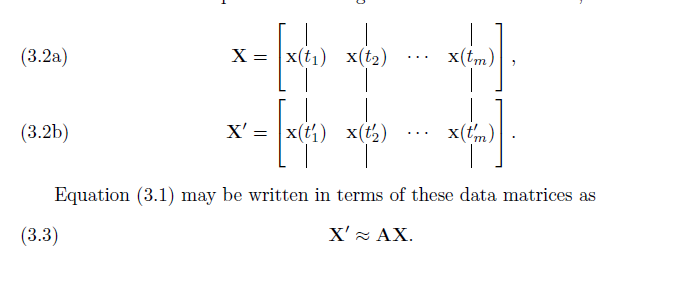
\includegraphics[scale=0.6]{../Figures/fig_dmd_fig1.png}
		%	\end{subfigure}
\end{figure}
\end{frame}

\begin{frame}{DMD trick}
\begin{figure}[h]
	\centering
	%	\begin{subfigure}{0.4\textwidth}
		%		\centering
		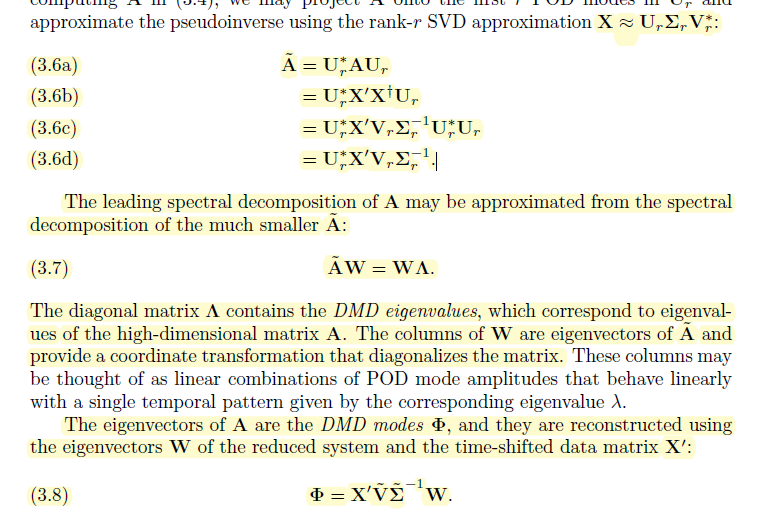
\includegraphics[scale=0.6]{../Figures/fig_dmd_fig2.png}
		%	\end{subfigure}
\end{figure}	
\end{frame}

\begin{frame}{DMD expansion}
\begin{figure}[h]
	\centering
	%	\begin{subfigure}{0.4\textwidth}
		%		\centering
		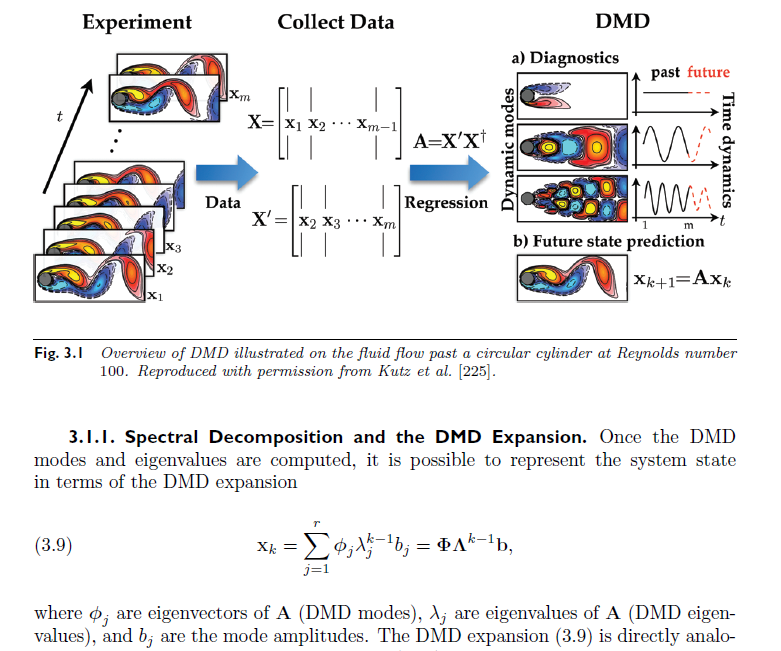
\includegraphics[scale=0.5]{../Figures/fig_dmd_fig3.png}
		%	\end{subfigure}
\end{figure}	
\end{frame}

\begin{frame}{DMD expansion (cont)}
	\begin{figure}[h]
		\centering
		%	\begin{subfigure}{0.4\textwidth}
			%		\centering
			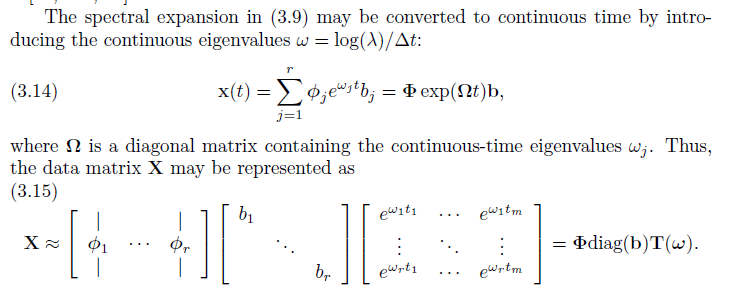
\includegraphics[scale=0.5]{../Figures/fig_dmd_fig4.png}
			%	\end{subfigure}
	\end{figure}	
\end{frame}


	
\begin{frame}{Colophon}
	\begin{figure}[h]
		\centering
		%	\begin{subfigure}{0.4\textwidth}
			%		\centering
			
\includegraphics[scale=0.35]{../Figures/siam_new.jpg}
			%	\end{subfigure}
	\end{figure}	
\end{frame}	



	%\begin{frame}{Fourier Transform}
	%	\begin{figure}[h]
		%	\centering
		%	%	\begin{subfigure}{0.4\textwidth}
			%		%		\centering
			%		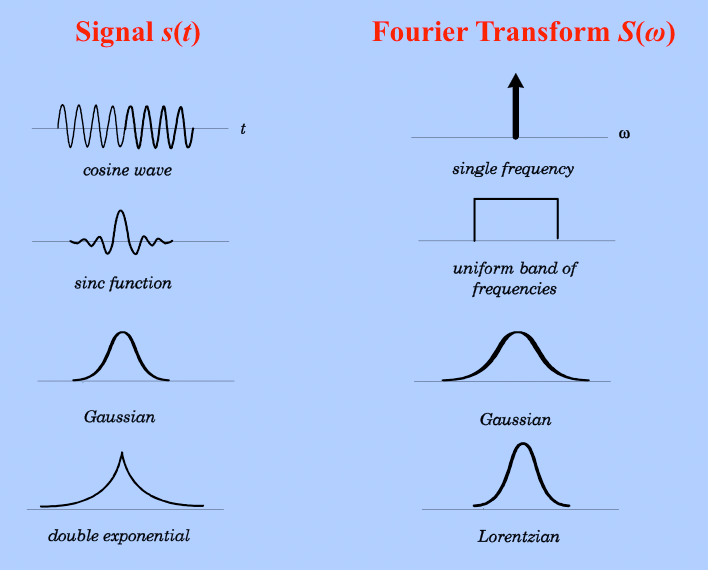
\includegraphics[scale=0.65]{../Figures/fig_fourier_transform.}
			%		%	\end{subfigure}
		%\end{figure}
		%\end{frame}
		
		
		%\begin{frame}{References}
		%	Materials and some of the pictures are from \citep{calin}.
		%	\printbibliography 	
		
		%	I have used some of the graphs by hacking TiKz code from StakExchange, Inkscape for more aesthetic plots and other old tricks of \TeX
		
		%\end{frame}
		
		
	\end{document}
